\section{규칙파 검증 실험 및 결과}

\subsection{조파기 구동 코드}

\begin{algorithm}[h]
    \caption{Sinusoidal Motion}
    \label{Sinusoidal Motion}
    \begin{algorithmic}[1]
    \Procedure{Sinusoidal Motion}{$A, N, \Delta\phi$}\Comment{Move the motor by sinusoidal function}
        \For{$elapsed Time \geq 0$}
            \If{$elapsed Time \geq N$}
                \State {$elapsed Time$ = 0}
                \State {$target = f(n)$}%\Comment{In this case, $target$ = $A \sin${($n$ $\Delta$$\phi$)}}
                % \State {$target$ = $A \sin${($n$ $\Delta$$\phi$)}}
                \State {$n$ $\gets$ $n$ + 1}
                \State {Move $motor$ to $target$}
            \EndIf
        \EndFor
        \EndProcedure
    \end{algorithmic}
\end{algorithm}

조파기 구동 코드는 시간간격 $N~\mathrm{ms}$마다 각 변위를 $f(n)$으로 지정한다 (알고리즘 \ref{Sinusoidal Motion}). 함수가 $\sin$이면 모터가 $\sin$ 각 변위를 따라 움직일 것으로 기대할 수 있다. $\sin$형 구동을 위한 코드의 $f(n)$은 다음과 같다.
\begin{equation}
    f(n) = A \sin(n \Delta\phi)
    \label{f(n)}
\end{equation}

실질적인 매개변수는 $A, \omega, N$이며 $A$는 진폭, $\omega$는 조파판 위상의 각진동수, $N$은 조파판의 변위를 업데이트하는 시간 간격이다. $\omega$는 다음과 같이 정의될 수 있다.
\begin{equation}
    \omega = \frac{\Delta\phi}{\Delta t} = \frac{\Delta\phi}{N}, ~\Delta\phi = N \omega
    \label{f(N)}
\end{equation}

$N$과 $\omega$가 매개된 입력 신호의 식이 실질적인 매개변수 표현이며 $A$와 $\omega$는 코드에서의 입력값과 조파기 구동 시 판의 움직임에서 실제로 나타나는 값이 달라 그 관계를 파악하기 위한 실험이 필수적이고 $\omega$가 너무 큰 경우 탈조가 날 수 있어 가능 범위를 파악해야 한다. $N$은 이론적으로 조파판의 움직임에 영향을 주지 않아 고정하여 실험을 진행했으나 판의 최대 변위와 최소 변위 지점에서 변위가 업데이트되어야 하므로 각진동수에 따른 $N$의 변화가 필요할 수 있다.

\subsection{예비 실험}
$A = 5\mathrm{~cm}$, $N=50$의 고정된 값에서 $\omega$를 $0.4\pi$에서 $\pi$까지 $0.1\pi$ 간격으로 변화시키며 실험하고 추가로 $1.5\pi$에 대해서도 실험했다.
판의 움직임을 분석했을 때 $\omega$가 증가함에 따라 진폭의 출력값이 감소하다. 생성파는 $\sin$파와 유사하였고 각진동수는 입력값과 동일했지만 진폭은 관계가 없어 실험 구성 단계에서는 모터의 움직임만 분석하였다.

\subsection{실험 구성}
생성파의 분석이 필요치 않으므로 조파기의 모터 대신 작은 모터에 회로를 연결하여 모터의 움직임이 $\sin$ 형태인지 확인하였다. 시리얼 모니터에 각 위치를 출력하여 알 수 있으며 출력값은 입력값과 일치하나 진폭은 달랐으며, $\omega$가 클수록 진폭의 출력값이 감소하였다. 즉, 파를 생성할 때 구동 코드의 매개변수에 따른 판의 움직임과 생성되는 파 2개를 관찰해야 하고 두 파의 진폭과 각진동수를 코드의 값과 비교하여 관계를 파악하는 것을 목표로 한다.

\begin{figure}[H]
    \centering
    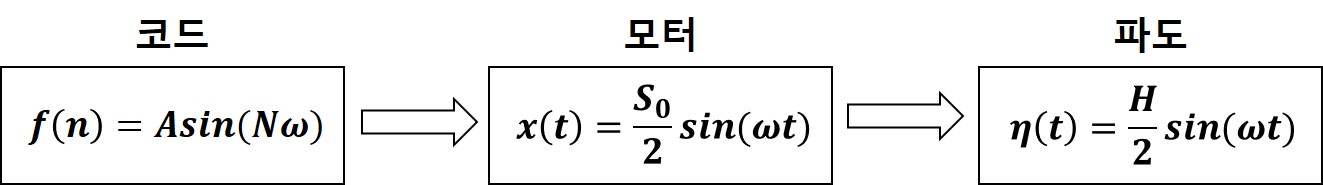
\includegraphics[width=12cm]{images/Flow_Chart(Analysis System_Kor).jpg}
    \caption{조파기 검증 실험의 흐름도}
    \label{Flow_Chart}
\end{figure}

$S_0$와 $A$의 직접적인 관계는 알 수 없으나 $S_0$와 $H$의 관계는 이론적 배경의 식을 따를 것으로 기대할 수 있으며 파가 $\sin$형이 아니더라도 FFT 분석을 통해서 $\omega$를 구할 수 있고 세 파동에서 일관될 것이다. 제대로 검증하기 위해서는 다양한 조건에 대한 데이터가 필요하며 이론적 분석과 예비 실험을 통해 정한 범위는 $A$는 $1\mathrm{~cm}$부터 $10\mathrm{~cm}$까지 $1\mathrm{~cm}$ 간격으로, $\omega$는 $3$부터 $12$까지 $1$ 간격으로 변화시키는 것이다. $N$은 50으로 고정시켰다 (단, 수심은 $15\mathrm{cm}$로 고정하였다).

%실험한 내용을 집어넣어야 함.

%실험계의 모식도가 필요함. 혹은 사진이라도.
\subsection{성능 검증 실험 결과}

% \begin{figure}[H]
%     \centering
%     \begin{tabular}{ll}
%         \begin{filecontents*}{A.dat}
% w_msr	A_thm	A_msr
% 0.6272	10	9.515
% 0.6275	10	9.532
% 0.6541	10	9.523
% 0.6681	10	9.499
% 0.6826	10	9.48
% 0.6978	10	9.456
% 0.6978	10	9.449
% 0.7849	10	9.326
% 0.785	10	9.318
% 0.8263	10	9.26
% 0.8971	10	9.138
% 0.8971	10	9.137
% 1.047	10	8.883
% 1.047	10	8.876
% 1.256	10	8.498
% 1.256	10	8.492
% 1.57	10	7.916
% 1.57	10	7.903
% 1.744	10	7.588
% 1.962	10	7.206
% 1.962	10	7.197
% 2.093	10	6.988
% 2.093	10	6.978
% 2.243	10	6.749
% 2.415	10	6.489
% 2.617	10	6.218
% 2.618   10	6.214
% 3.141	10	4.837
% 3.141	10	4.837
% 3.927	10	3.093
% 5.236	10	0.5795
%         \end{filecontents*}

%         \begin{tikzpicture}[
%                 %Environment Cfg.
%                 %font=\bfseries\sffamily,
%             ]
%             \begin{axis}[
%                 width=6cm,
%                 height=6cm,
%                 at={(0,0)},
%                 ymin=0,
%                 ymax=13,
%                 xmin=0,
%                 xmax=6,
%                 grid=both,
%                 minor tick num =5,
%                 minor tick style={draw=none},
%                 minor grid style={thin,color=black!10},
%                 major grid style={thin,color=black!10},
%                 %ylabel style={rotate=90},
%                 ylabel={$A_{plate}~\left[\mathrm{~cm}\right]$},
%                 xlabel={$\omega_{msr}~\left[\mathrm{~rad/s}\right]$},
%                 tick align=outside,
%                 axis x line*=middle,
%                 axis y line*=none,
%                 xtick={0,2,...,16},
%                 ytick={0,2,...,16},
%                 %xlabel style={color=blue!50!cyan},
%                 %ylabel style={align=center,rotate=-90,color=blue!50!cyan},
%                 x tick label style={
%                     /pgf/number format/assume math mode, font=\sf\scriptsize},
%                 y tick label style={
%                     /pgf/number format/assume math mode, font=\sf\scriptsize},
%                 legend cell align = {left},
%                 legend pos = north west,
%                 legend style={nodes={scale=0.5, transform shape}},
%                 ]
%                 \addplot [%only marks, 
%                     mark size=1pt,
%                     mark=o, 
%                     %mark options={solid}, 
%                     %smooth,
%                     ] 
%                 table [x=w_msr, y=A_thm] {A.dat};
%                 \addlegendentry{$A_{thm} - \omega_{msr}$}
%                 \addplot [%only marks, 
%                     mark = +,
%                     mark size=1pt,
%                     ]
%                 table [x=w_msr, y=A_msr] {A.dat};
%                 \addlegendentry{$A_{msr} - \omega_{msr}$}
%             \end{axis}
%         \end{tikzpicture}
        
%         &
        
%         \begin{filecontents}{B.dat}
%                     wthm   wPlate
% 0.6283	0.6272
% 0.6981	0.6978
% 0.7854	0.785
% 0.8976	0.8971
% 1.0472	1.047
% 1.2566	1.256
% 1.5708	1.57
% 1.9635	1.962
% 2.0944	2.093
% 2.6180	2.617
% 3.1416	3.141
% 3.9270	3.918
% 5.2360	5.236
% 4.4880	4.487
% 3.9270	3.919
% 3.4907	3.49
% 0.6283	0.6275
% 0.6545	0.6541
% 0.6684	0.6681
% 0.6830	0.6826
% 0.6981	0.6978
% 0.7854	0.7849
% 0.8267	0.8263
% 0.8976	0.8971
% 1.0472	1.047
% 1.2566	1.256
% 1.5708	1.57
% 1.7453	1.744
% 1.9635	1.962
% 2.0944	2.093
% 2.2440	2.243
% 2.4166	2.415
% 2.6180	2.617
% 3.1416	3.141
%             \end{filecontents}
        
%             \begin{tikzpicture}[
%                     %Environment Cfg.
%                     font=\bfseries\sffamily,
%                 ]
%                     \begin{axis}[
%                         width=6cm,
%                         height=6cm,
%                         at={(0,0)},
%                         ymin=0,
%                         ymax=6,
%                         xmin=0,
%                         xmax=6,
%                         grid=both,
%                         minor tick num =5,
%                         minor tick style={draw=none},
%                         minor grid style={thin,color=black!10},
%                         major grid style={thin,color=black!10},
%                         %ylabel style={rotate=90},
%                         ylabel={$\omega_{msr}~\left[\mathrm{rad/s}\right]$},
%                         xlabel={$\omega_{thm}~\left[\mathrm{rad/s}\right]$},
%                         tick align=outside,
%                         axis x line*=middle,
%                         axis y line*=none,
%                         xtick={0,2,...,16},
%                         ytick={0,2,...,16},
%                         %xlabel style={color=blue!50!cyan},
%                         %ylabel style={align=center,rotate=-90,color=blue!50!cyan},
%                         x tick label style={
%                             /pgf/number format/assume math mode, font=\sf\scriptsize},
%                         y tick label style={
%                         /pgf/number format/assume math mode, font=\sf\scriptsize},
%                         legend cell align = {left},
%                         legend pos = north west,
%                         legend style={nodes={scale=0.5, transform shape}},
%                         ]
%                         \addplot [only marks, 
%                             mark size=1pt,
%                             mark=o, 
%                             ]
%                             table [x=wthm, y=wPlate] {B.dat};
%                            \addlegendentry{$ \omega_{msr} - \omega_{thm}$}
%                     \end{axis}
%         \end{tikzpicture}
%     \end{tabular}
    
%     \begin{tikzpicture} [remember picture, overlay]
%         \node at (-5.8, 0.6) {\scriptsize{(a)}};
%         \node at (2.0, 0.6) {\scriptsize{(b)}};
%     \end{tikzpicture}
%     \caption{$\omega_{msr} - \omega_{thm}$ graph - (a) wave (b) plate}
%     \label{PreExperiment}
% \end{figure}


%%%%%%%%%%%%%%%%%%%%%%%% 없애버려야 할 엑셀 사진들 %%%%%%%%%%%%%%%%%%%%%%%%%
% \begin{figure}[H]
%     \centering
%     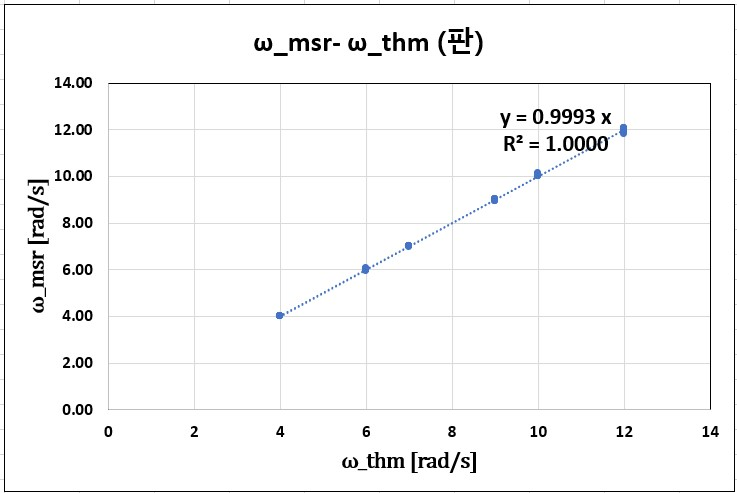
\includegraphics[height=5cm]{images/Experiment(omega_thm-omega_msr)_Plate_Kor.jpg}
%     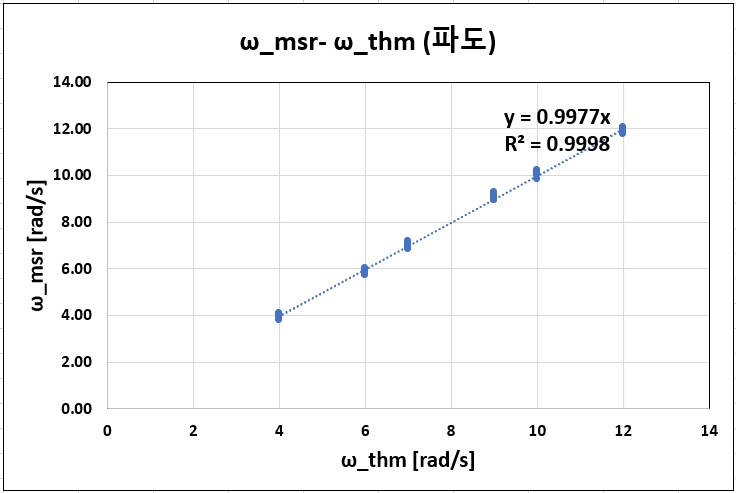
\includegraphics[height=5cm]{images/Experiment(omega_thm-omega_msr)_Wave_Kor.jpg}
%     \caption{측정한 $\omega_{msr}$에 대한 코드의 $\omega_{thm}$ (좌),  $\omega_{msr}$에 대한 측정 진폭 $A_{msr}$ (우) - 검증 실험}
%     \label{ExperimentGraph - 1, 2}
% \end{figure}
%%%%%%%%%%%%%%%%%%%%%%%%%%%%%%%%%%%%%%%%%%%%%%%%%%%%%%%%%%%%%%%%%%%%%%%%%

\begin{figure}[htbp]
    \centering
    \begin{tabular}{ll}
        \begin{filecontents*}{wthm-wwave.dat}
            wthm    wwave
            12  12.03
            12	11.91
            12	11.88
            12	11.96
            12	12.07
            12	12
            12	11.8
            12	12
            12	11.9
            12	11.77
            10	10.2
            10	10.1
            10	10.01
            10	10.07
            10	10.1
            10	10.07
            10	10.09
            10	10.05
            10	10.15
            10	9.84
            9	8.95
            9	9.02
            9	9
            9	9.02
            9	9.15
            9	9.28
            9	9.17
            9	8.94
            9	8.94
            9	8.94
            7	7.16
            7	6.99
            7	6.86
            7	6.99
            7	6.89
            7	6.85
            7	7.06
            7	6.89
            7	6.91
            7	6.9
            6	5.93
            6	5.96
            6	5.97
            6	5.94
            6	6.03
            6	5.73
            6	5.77
            6	5.76
            6	5.94
            6	5.79
            4	3.908
            4	3.984
            4	3.969
            4	3.982
            4	3.978
            4	4.082
            4	4.025
            4	4.051
            4	3.86
            4	3.784            
        \end{filecontents*}
    
        \begin{tikzpicture}[
                %Environment Cfg.
                %font=\bfseries\sffamily,
            ]
            \begin{axis}[
                width=8cm,
                height=8cm,
                at={(0,0)},
                ymin=0,
                ymax=15,
                xmin=0,
                xmax=15,
                grid=both,
                minor tick num =5,
                minor tick style={draw=none},
                minor grid style={thin,color=black!10},
                major grid style={thin,color=black!10},
                %ylabel style={rotate=90},
                ylabel={$\omega_{msr}~\left[\mathrm{rad}/s\right]$},
                xlabel={$\omega_{thm}~\left[\mathrm{rad}/s\right]$},
                tick align=outside,
                axis x line*=middle,
                axis y line*=none,
                xtick={0,2,...,16},
                ytick={0,2,...,16},
                %xlabel style={color=blue!50!cyan},
                %ylabel style={align=center,rotate=-90,color=blue!50!cyan},
                x tick label style={
                    /pgf/number format/assume math mode, font=\scriptsize},
                y tick label style={
                    /pgf/number format/assume math mode, font=\scriptsize},
                legend cell align = {left},
                legend pos = north west,
                legend style={nodes={scale=0.75, transform shape}},
                ]
                \addplot [only marks, 
                    mark size=1pt,
                    mark=o, 
                    %mark options={solid}, 
                    %smooth,
                    ] 
                    table [x=wthm, y=wwave] {wthm-wwave.dat};
                \addlegendentry{$ \omega_{msr}(wave) - \omega_{thm}$}
                \addplot [thick, red] table [y={create col/linear regression={y=wwave}}] {wthm-wwave.dat};
                \addlegendentry{
                    Linear regression: $ \omega_{msr} =
                    \pgfmathprintnumber{\pgfplotstableregressiona}
                    \cdot \omega_{thm}
                    \pgfmathprintnumber[print sign]{\pgfplotstableregressionb}$
                    };

                % \addplot[color=blue!50!cyan,smooth,tension=0.7,very thick] table [x index=0,y index=1,col sep=space] {Aplate-wmsrS.dat};
                % \addplot[color=cyan!50!lime,very thick] coordinates{(0,5)(25,5)};
                % \addplot[color=orange,very thick] coordinates{(0,11)(25,11)};
                % \addplot[color=red!80!orange,very thick] coordinates{(19,24.2)(23,24.2)};
                % \node[text=cyan!50!lime,fill=white,align=center,anchor=west,scale=0.8,inner sep=5pt] at (24.5,5){Base\\ Load};
                % \node[color=orange,fill=white,align=center,anchor=west,scale=0.8,inner sep=5pt] at (24.5,11){Average\\ Load};
                % \node[color=red!80!orange,fill=white,align=center,anchor=west,scale=0.8,inner sep=5pt] at (21.2,24.2){Maxium\\ Load};
            \end{axis}
        \end{tikzpicture}
        
        &
        
        \begin{filecontents}{wthm-wplate.dat}
                    wthm   wPlate
                    12	12.00
                    12	12.04
                    12	12.06
                    12	12.01
                    12	11.81
                    12	12.06
                    12	11.88
                    12	11.98
                    12	11.89
                    12	11.95
                    10	10.00
                    10	10.06
                    10	10.04
                    10	10.05
                    10	9.99
                    10	10.14
                    10	9.99
                    10	10.00
                    10	10.10
                    10	9.99
                    9	9.00
                    9	9.00
                    9	8.98
                    9	8.99
                    9	8.93
                    9	8.95
                    9	8.91
                    9	9.00
                    9	8.99
                    9	9.00
                    7	7.00
                    7	7.00
                    7	7.00
                    7	7.00
                    7	7.00
                    7	6.99
                    7	7.00
                    7	6.99
                    7	7.00
                    7	6.98
                    6	6.00
                    6	6.00
                    6	5.99
                    6	6.01
                    6	5.94
                    6	5.99
                    6	6.00
                    6	6.00
                    6	6.04
                    6	6.05
                    4	4
                    4	4
                    4	4.001
                    4	4.001
                    4	4.001
                    4	4.001
                    4	4
                    4	4
                    4	4.001
                    4	4.001   
            \end{filecontents}
        
            \begin{tikzpicture}[
                    %Environment Cfg.
                    font=\bfseries\sffamily,
                ]
                    \begin{axis}[
                        width=8cm,
                        height=8cm,
                        at={(0,0)},
                        ymin=0,
                        ymax=15,
                        xmin=0,
                        xmax=15,
                        grid=both,
                        minor tick num =5,
                        minor tick style={draw=none},
                        minor grid style={thin,color=black!10},
                        major grid style={thin,color=black!10},
                        %ylabel style={rotate=90},
                        ylabel={$\omega_{msr}~\left[\mathrm{rad}/s\right]$},
                        xlabel={$\omega_{thm}~\left[\mathrm{rad}/s\right]$},
                        tick align=outside,
                        axis x line*=middle,
                        axis y line*=none,
                        xtick={0,2,...,16},
                        ytick={0,2,...,16},
                        %xlabel style={color=blue!50!cyan},
                        %ylabel style={align=center,rotate=-90,color=blue!50!cyan},
                        x tick label style={
                            /pgf/number format/assume math mode}, %, font=\scriptsize
                        y tick label style={
                        /pgf/number format/assume math mode}, %, font=\sf\scriptsize
                        legend cell align = {left},
                        legend pos = north west,
                        legend style={nodes={scale=0.75, transform shape}},
                        ]
                        \addplot [only marks, 
                            mark size=1pt,
                            mark=o, 
                            ]
                            table [x=wthm, y=wPlate] {wthm-wplate.dat};
                        \addplot [thick, red] table [y={create col/linear regression={y=wPlate}}] {wthm-wplate.dat};
                        \addlegendentry{$ \omega_{msr}(plate) - \omega_{thm}$}
                        \addlegendentry{
                            Linear regression: $ \omega_{msr} =
                            \pgfmathprintnumber{\pgfplotstableregressiona}
                            \cdot \omega_{thm}
                            \pgfmathprintnumber[print sign]{\pgfplotstableregressionb}$
                        };

                        % \addplot[color=blue!50!cyan,smooth,tension=0.7,very thick] table [x index=0,y index=1,col sep=space] {Aplate-wmsrS.dat};
                        % \addplot[color=cyan!50!lime,very thick] coordinates{(0,5)(25,5)};
                        % \addplot[color=orange,very thick] coordinates{(0,11)(25,11)};
                        % \addplot[color=red!80!orange,very thick] coordinates{(19,24.2)(23,24.2)};
                        % \node[text=cyan!50!lime,fill=white,align=center,anchor=west,scale=0.8,inner sep=5pt] at (24.5,5){Base\\ Load};
                        % \node[color=orange,fill=white,align=center,anchor=west,scale=0.8,inner sep=5pt] at (24.5,11){Average\\ Load};
                        % \node[color=red!80!orange,fill=white,align=center,anchor=west,scale=0.8,inner sep=5pt] at (21.2,24.2){Maxium\\ Load};
                    \end{axis}
        \end{tikzpicture}
    \end{tabular}
    \begin{tikzpicture} [remember picture, overlay]
        \node at (-14.8, -3.5) {{(a)}};
        \node at (-6.7, -3.5) {{(b)}};
    \end{tikzpicture}
    \caption{$\omega_{msr} - \omega_{thm}$ 그래프- (a) 파도 (b) 조파판}
    \label{Experiment: omega - omega graph}
\end{figure}

그림 \ref{Experiment: omega - omega graph}에서 알 수 있듯이 $\omega$는 코드에서 대입한 값과 판, 파도 모두 같은 값을 띔을 알 수 있다 (두 그래프 모두 선형 관계를 만족하며($R^2 > 0.99$) 그 기울기는 약 1.000이다). 또, 분산 관계식과 식 \ref{eq:5}을 통해 주어진 $\omega$에 대한 $H/S$를 예측할 수 있고 이를 측정값과 비교해보았다.

%%%%%%%%%%%%%%%%%%%%%%%%% 없애버려야 할 엑셀 사진 %%%%%%%%%%%%%%%%%%%%%%%%%
% \begin{figure}[H]
%     \centering
%     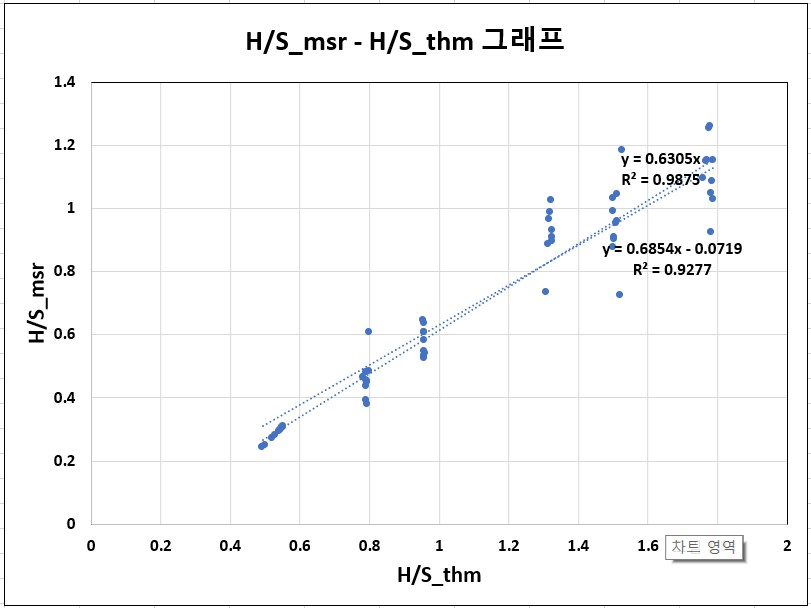
\includegraphics[width=0.70\textwidth]{images/Experiment(H.S_thm-H.S_msr).jpg}
%     \caption{$H/S_{msr} - H/S_{thm}$ 그래프}
%     \label{H/S Graph}
% \end{figure}
%%%%%%%%%%%%%%%%%%%%%%%%%%%%%%%%%%%%%%%%%%%%%%%%%%%%%%%%%%%%%%%%%%%%%%%%%

\begin{figure}[H]
    \centering
        \begin{filecontents}{HSthm-HSmsr.dat}
                HS_thm	HS_msr
                1.781440728	0.925436527
                1.785651376	1.085170025
                1.787735635	1.027713311
                1.782498659	1.045913291
                1.760671425	1.094309648
                1.787735635	1.15104453
                1.768471166	1.150212766
                1.77931432	1.26011236
                1.769571325	1.151819856
                1.776098332	1.252500343
                1.502818971	0.907053163
                1.512879552	1.042827713
                1.509535179	0.952282833
                1.51120852	0.957989748
                1.501134272	0.989520132
                1.526163172	1.182451424
                1.501302842	1.031007752
                1.502482211	0.900403351
                1.519540335	0.724198251
                1.501134272	0.877353529
                1.324569679	0.909190732
                1.324937643	0.929155313
                1.321072373	0.986915888
                1.323465588	1.024621212
                1.313331279	0.887096774
                1.315913161	0.964838394
                1.309086454	0.733436773
                1.326041332	0.895167286
                0.958556795	0.531089978
                0.958906454	0.580898876
                0.959081306	0.608042895
                0.958731617	0.530870712
                0.959081306	0.635545557
                0.956634768	0.607395324
                0.959431056	0.540311804
                0.95646013	0.524718468
                0.958556795	0.547893826
                0.954714602	0.645610278
                0.792888221	0.451327434
                0.792888221	0.377926685
                0.790392394	0.481381958
                0.793981875	0.44980695
                0.783557379	0.464839094
                0.791639619	0.434911243
                0.792419834	0.455155071
                0.79195164	0.393355983
                0.798366989	0.608601216
                0.800094292	0.48515625
                0.492276411	0.242943759
                0.528893957	0.280658651
                0.543862815	0.296883754
                0.553908234	0.308036891
                0.552905492	0.306913997
                0.542089448	0.294936947
                0.546948794	0.300287356
                0.551047756	0.304839279
                0.521368486	0.272679232
                0.499818992	0.25048407                  
            \end{filecontents}
        
            \begin{tikzpicture}[
                    %Environment Cfg.
                    font=\bfseries\sffamily,
                ]
                    \begin{axis}[
                        width=16cm,
                        height=8cm,
                        at={(0,0)},
                        ymin=0,
                        ymax=1.4,
                        xmin=0,
                        xmax=2,
                        grid=both,
                        minor tick num =5,
                        minor tick style={draw=none},
                        minor grid style={thin,color=black!10},
                        major grid style={thin,color=black!10},
                        %ylabel style={rotate=90},
                        ylabel={$H/S_{msr}$},
                        xlabel={$H/S_{thm}$},
                        tick align=outside,
                        axis x line*=middle,
                        axis y line*=none,
                        xtick={0,0.2,...,2},
                        ytick={0,0.2,...,2},
                        %xlabel style={color=blue!50!cyan},
                        %ylabel style={align=center,rotate=-90,color=blue!50!cyan},
                       x tick label style={
                            /pgf/number format/assume math mode, font=\sf\scriptsize},
                        y tick label style={
                            /pgf/number format/assume math mode, font=\sf\scriptsize},
                        legend cell align = {left},
                        legend pos = north west,
                        legend style={nodes={scale=1, transform shape}},
                        ]
                        \addplot[scatter, 
                                only marks, 
                                mark=o,
                                mark size=1.5pt,
                                color=black,
                            ] 
                        table [x=HS_thm, y=HS_msr]{HSthm-HSmsr.dat};    
                        \addplot [thick, red] table [y={create col/linear regression={y=HS_msr}}] {HSthm-HSmsr.dat};
                        %\addlegendentry{$y(x)$}
                        \addlegendentry{
                            Linear regression: $ \omega_{msr} =
                            \pgfmathprintnumber{\pgfplotstableregressiona}
                            \cdot \omega_{thm}
                            \pgfmathprintnumber[print sign]{\pgfplotstableregressionb}$
                        };

                        % \addplot[color=blue!50!cyan,smooth,tension=0.7,very thick] table [x index=0,y index=1,col sep=space] {Aplate-wmsrS.dat};
                        % \addplot[color=cyan!50!lime,very thick] coordinates{(0,5)(25,5)};
                        % \addplot[color=orange,very thick] coordinates{(0,11)(25,11)};
                        % \addplot[color=red!80!orange,very thick] coordinates{(19,24.2)(23,24.2)};
                        % \node[text=cyan!50!lime,fill=white,align=center,anchor=west,scale=0.8,inner sep=5pt] at (24.5,5){Base\\ Load};
                        % \node[color=orange,fill=white,align=center,anchor=west,scale=0.8,inner sep=5pt] at (24.5,11){Average\\ Load};
                        % \node[color=red!80!orange,fill=white,align=center,anchor=west,scale=0.8,inner sep=5pt] at (21.2,24.2){Maxium\\ Load};
                    \end{axis}
        \end{tikzpicture}
    \caption{$H/S_{msr} - H/S_{thm}$ graph}
    \label{H/S graph}
\end{figure}

$H/S$는 선형 관계를 만족한다고 볼 수 있다 (그림 \ref{H/S graph}). 측정값이 구간으로 나타났으나 이는 불확도 내의 값으로 취급할 수 있으며 선형 추세선의 기울기가 $1.000$은 아니지만 선형 추세를 통해 매개변수로부터 $H/S$를 예측할 수 있다.

% \begin{figure}[H]
%     \centering
%     % 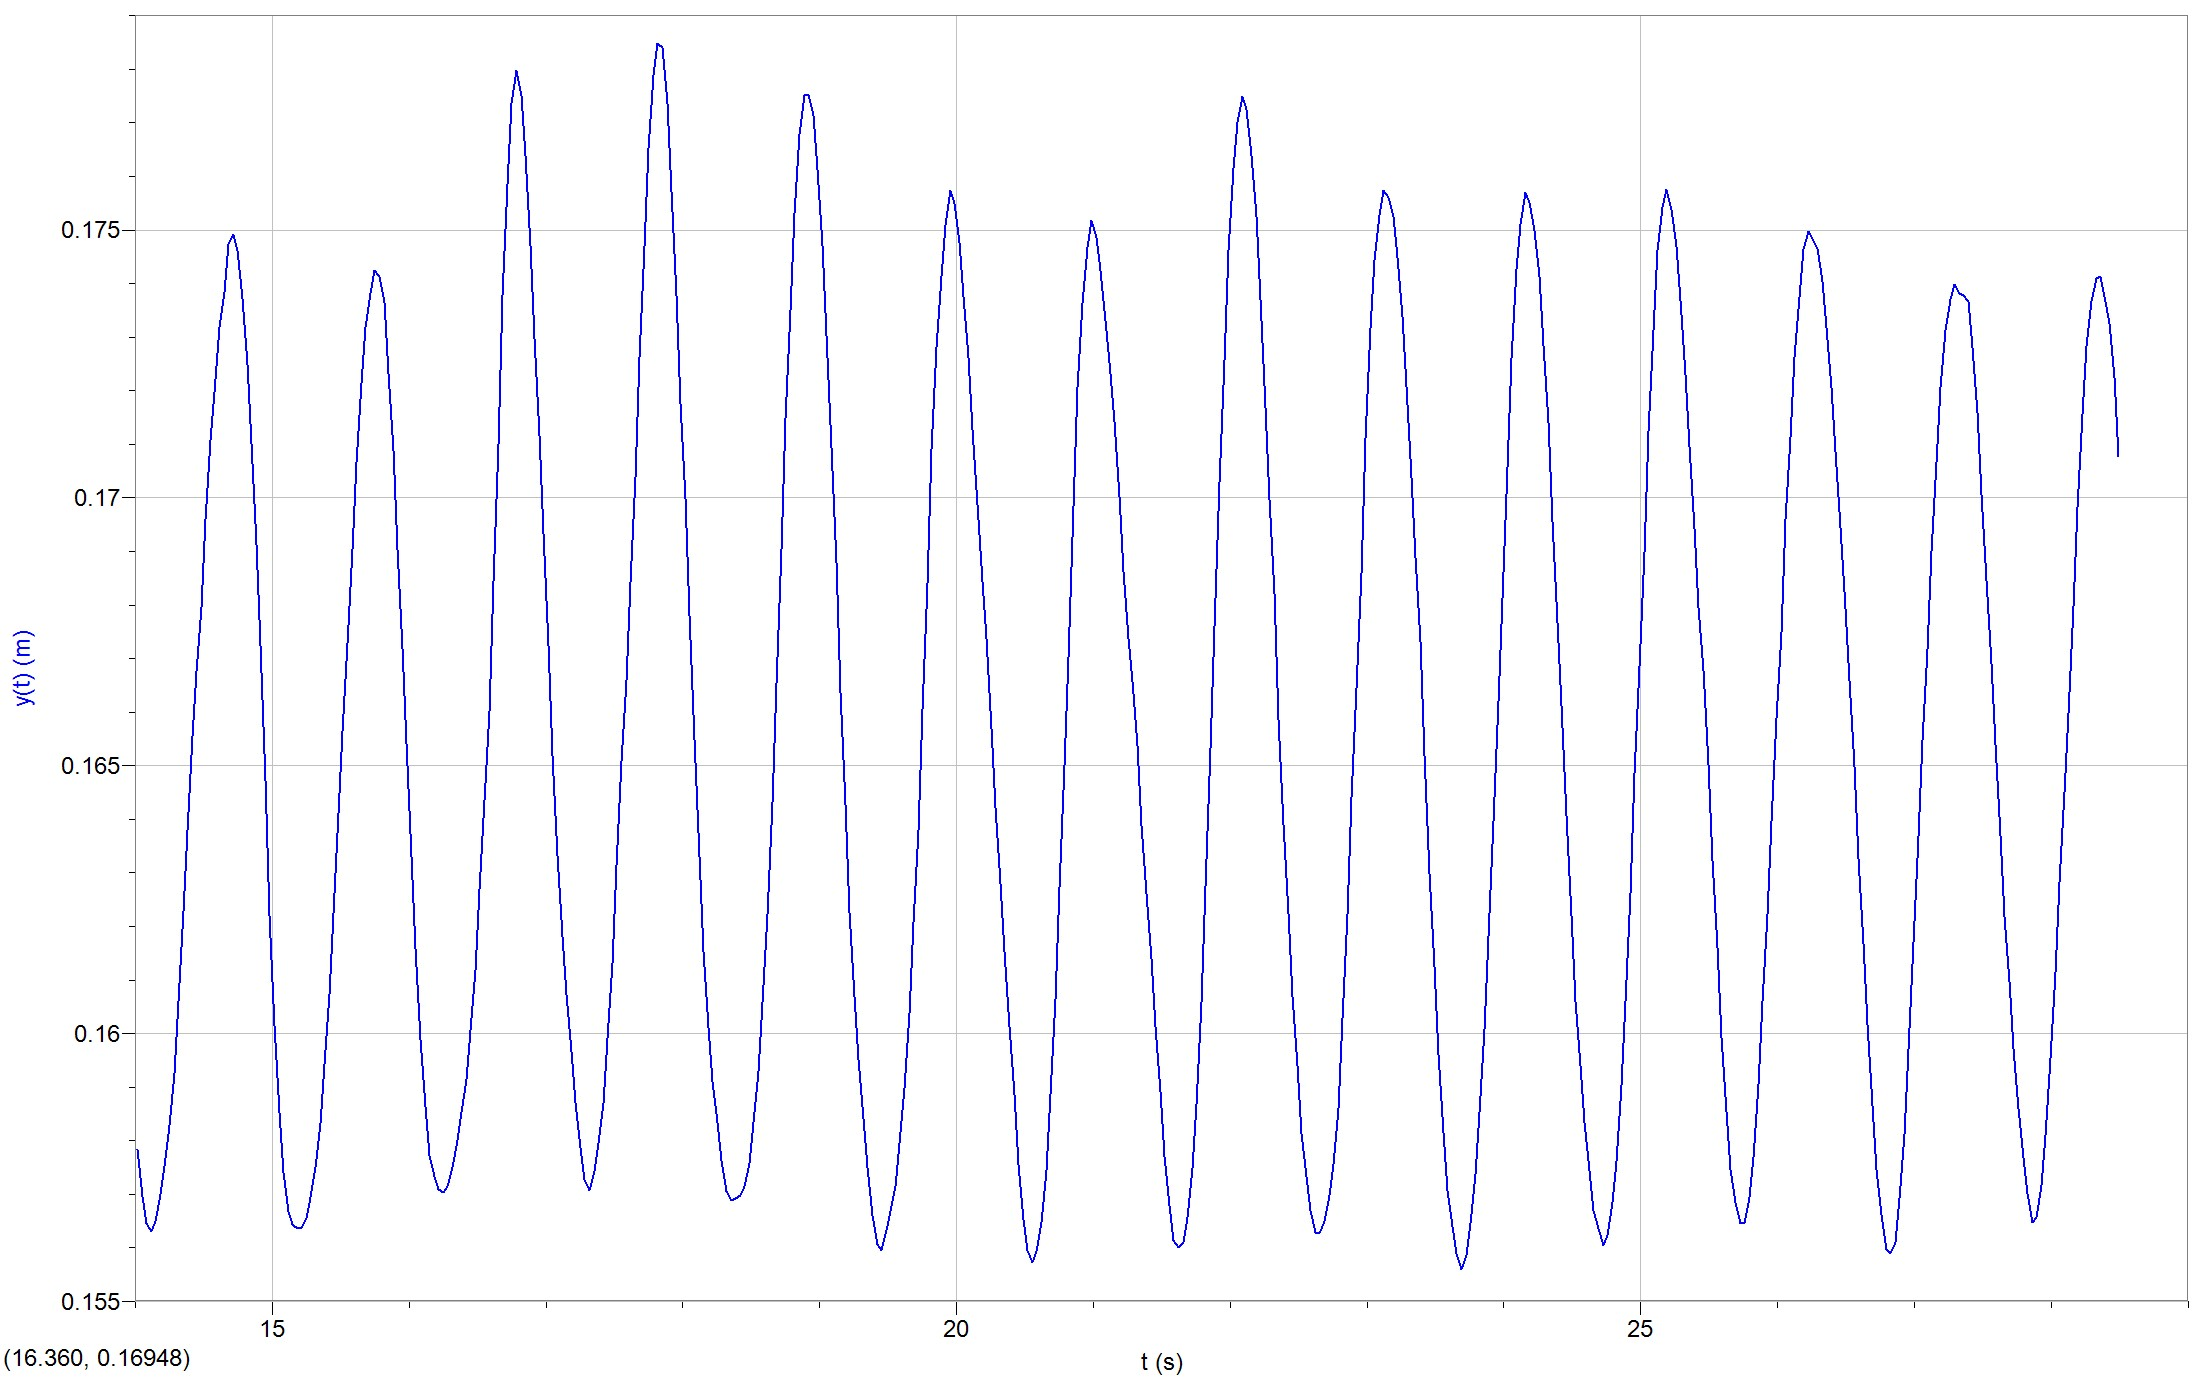
\includegraphics[width=0.70\textwidth]{images/Wave(omega=6,A=2).jpg}
%     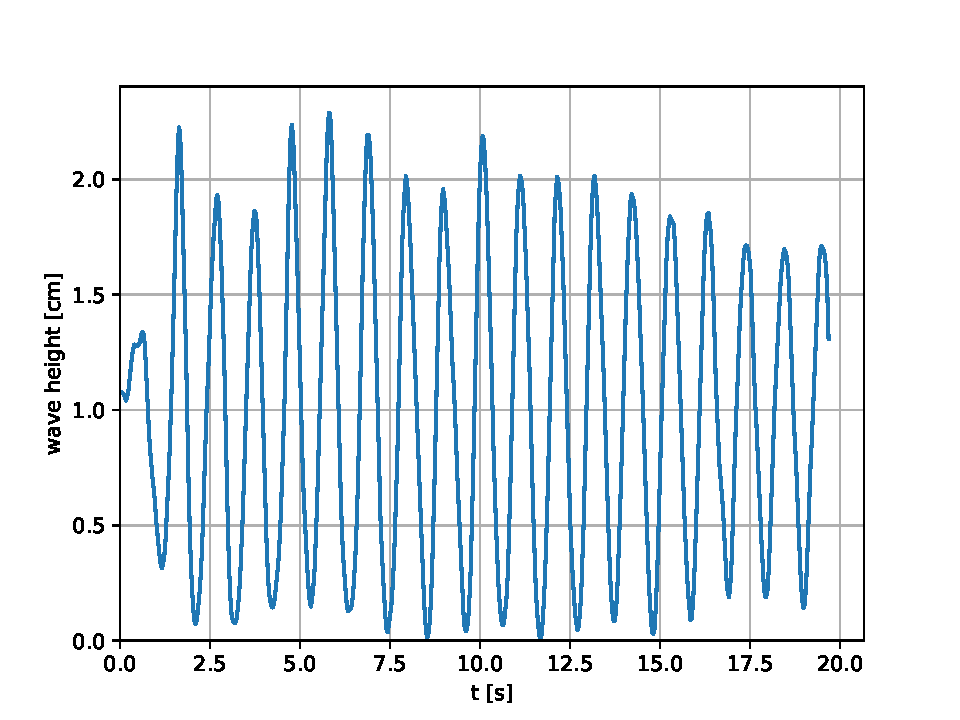
\includegraphics[width=0.70\textwidth]{images/omega=2.00_A=2_wave.pdf}
%     \caption{파형 데이터($A=2\mathrm{~cm},~\omega=6\mathrm{~rad/s}$)}
%     \label{Example Wave Data}
% \end{figure}

% 그림 \ref{Example Wave Data}는 한 sin 파의 예시이다. 코드에서는 $A=2\mathrm{~cm},~\omega=6\mathrm{rad/s}$를 대입하였으며 측정값은 $A=0.9588\mathrm{~cm},~\omega=5.959\mathrm{~rad/s}$이다. 

\subsection{오차 원인}

본 실험에서는 실험 과정에서의 오차, 분석 상의 오차 등 여러 오차가 존재한다. 이는 크게 모터에 의한 것과 파고계 영상 분석에 의한 것으로 나눌 수 있다.

모터의 한계에 의해 $\omega$에 따른 $A$의 한계와 아두이노에서 업로드한 파의 형태에 오차가 생긴다. 최대 각가속도가 판 움직임의 진폭과 오차를 결정한다는 것은 실험을 통해 알 수 있었으며 $\omega = 6$, $A = 5\mathrm{~cm}$의 고정된 상태에서 각가속도만 $30,000\mathrm{~step/s^2}$, $40,000\mathrm{~step/s^2}$, $50,000\mathrm{~step/s^2}$로 바꿔가며 판의 움직임을 분석하였다. 판 움직임을 정렬한 결과가 그림 \ref{fig:diffa}이다. $x$축은 시간이고 $y$축은 판의 변위($\mathrm{~m}$)이고 눈금 한 개의 스케일은 $0.01\mathrm{~m}$이다.

\begin{figure}[H]
    \centering
        \begin{filecontents}{acc.dat}
                t	y_30000	y_40000	y_50000
                0	0.19965	-0.0461	-0.70283
                0.033367	0.88578	0.79731	0.26519
                0.066734	1.41854	1.54643	1.3542
                0.1001	1.78019	2.09436	2.16649
                0.133467	2.10058	2.51832	2.74721
                0.166834	2.42496	2.9166	3.28632
                0.2002	2.65052	3.25279	3.73685
                0.233567	2.69128	3.32493	3.95223
                0.266934	2.69601	3.32011	4.0169
                0.3003	2.68381	3.31722	4.04341
                0.333667	2.53945	3.18505	3.92908
                0.367034	2.24984	2.85109	3.62093
                0.4004	1.94568	2.46075	3.19471
                0.433767	1.6103	2.00279	2.6843
                0.467134	1.14521	1.38601	1.98441
                0.5005	0.55864	0.64207	1.11098
                0.533867	-0.0586	-0.14149	0.16794
                0.567234	-0.68693	-0.94865	-0.8004
                0.6006	-1.16272	-1.669	-1.63958
                0.633967	-1.51151	-2.20274	-2.34206
                0.667334	-1.86959	-2.67197	-3.00563
                0.7007	-2.15706	-3.05802	-3.48397
                0.734067	-2.2686	-3.25109	-3.80335
                0.767434	-2.3295	-3.3759	-4.05893
                0.8008	-2.3925	-3.44363	-4.18022
                0.834167	-2.34221	-3.34345	-4.09689
                0.867534	-2.12824	-3.09611	-3.91013
                0.9009	-1.92868	-2.80851	-3.63691
                0.934267	-1.66742	-2.44389	-3.16259
                0.967634	-1.20691	-1.87777	-2.55154
                1.001	-0.71952	-1.22286	-1.84435
                1.034367	-0.20613	-0.50127	-1.04396
                1.067734	0.42368	0.31501	-0.09588
                1.1011	1.05093	1.12604	0.91296
                1.134467	1.51691	1.75337	1.7925
                1.167834	1.85038	2.20687	2.43867
                1.2012	2.15589	2.58406	3.00982
                1.234567	2.44035	2.96622	3.51607
                1.267934	2.55892	3.18147	3.8099
                1.3013	2.58132	3.1805	3.92574
                1.334667	2.58654	3.18082	3.99092
                1.368034	2.50032	3.12393	3.96888
                1.4014	2.27759	2.85251	3.70347
                1.434767	2.01037	2.44489	3.35212
                1.468134	1.70864	2.02859	2.9192
                1.5015	1.27966	1.48942	2.28589
                1.534867	0.72957	0.7975	1.52725
                1.568234	0.13968	-0.00332	0.65856
                1.6016	-0.46007	-0.82565	-0.34092
                1.634967	-1.00343	-1.61238	-1.27387
                1.668334	-1.39078	-2.12874	-1.98071
                1.7017	-1.73618	-2.63824	-2.67774
                1.735067	-2.05872	-3.06711	-3.25502
                1.768434	-2.2378	-3.33038	-3.59615
                1.8018	-2.28124	-3.46167	-3.88219
                1.835167	-2.35317	-3.55984	-4.08709
                1.868534	-2.34231	-3.52169	-4.05134
                1.9019	-2.18136	-3.3411	-3.88661
                1.935267	-1.96749	-3.06891	-3.67773
                1.968634	-1.71625	-2.72452	-3.26969
                2.002	-1.28602	-2.2191	-2.70558
                2.035367	-0.81728	-1.55728	-2.02746
                2.068734	-0.31872	-0.84745	-1.2709
                2.1021	0.26265	-0.07845	-0.30425
                2.135467	0.9496	0.788	0.72003
                2.168834	1.40154	1.52533	1.62134
                2.2022	1.75468	2.01573	2.30078
                2.235567	2.10147	2.46746	2.94581
                2.268934	2.3967	2.87079	3.47737
                2.3023	2.55238	3.15844	3.81726
                2.335667	2.62076	3.23622	4.00602
                2.369034	2.65914	3.27771	4.14932
                2.4024	2.58367	3.24675	4.15548
                2.435767	2.39857	3.05535	3.94408
                2.469134	2.17446	2.71809	3.62721
                2.5025	1.88444	2.34949	3.25509
                2.535867	1.49925	1.85688	2.65401
                2.569234	1.00332	1.21929	1.93541
                2.6026	0.44518	0.50017	1.14535
                2.635967	-0.19936	-0.3095	0.13966
                2.669334	-0.74776	-1.08519	-0.83255
                2.7027	-1.20231	-1.64584	-1.61405
                2.736067	-1.59977	-2.20759	-2.37864
                2.769434	-1.93983	-2.65238	-3.00176
                2.8028	-2.17932	-2.94288	-3.4264
                2.836167	-2.29458	-3.10488	-3.73815
                2.869534	-2.37942	-3.21108	-3.99138
                2.9029	-2.38288	-3.20642	-4.04015
                2.936267	-2.27697	-3.0282	-3.91074
                2.969634	-2.1216	-2.7839	-3.74705
                3.003	-1.91887	-2.45772	-3.3983
                3.036367	-1.55399	-1.99512	-2.917
                3.069734	-1.07152	-1.35359	-2.28586
                3.1031	-0.64736	-0.69868	-1.56226
                3.136467	-0.07503	0.07567	-0.67443
                3.169834	0.62139	0.96725	0.30019
                3.2032	1.15329	1.72133	1.32913
                3.236567	1.52816	2.28082	2.12527
                3.269934	1.89348	2.70848	2.72048
                3.3033	2.24371	3.18353	3.26412
                3.336667	2.43633	3.40231	3.70057
                3.370034	2.53906	3.47484	3.94051
                3.4034	2.60009	3.55977	4.05245
                3.436767	2.56799	3.57702	4.09095
                3.470134	2.42036	3.37121	3.96946
                3.5035	2.20923	3.07584	3.65483
                3.536867	1.93066	2.78252	3.2648
                3.570234	1.55913	2.26567	2.78462
                3.6036	1.10325	1.61979	2.07279
                3.636967	0.5802	0.97997	1.24147
                3.670334	-0.02334	0.17924	0.34297
                3.7037	-0.65857	-0.75173	-0.64667
                3.737067	-1.17285	-1.37792	-1.55053
                3.770434	-1.56799	-1.91885	-2.26503
                3.8038	-1.90164	-2.46202	-2.94488
                3.837167	-2.23698	-2.85342	-3.50423
                3.870534	-2.44391	-3.05384	-3.83199
                3.9039	-2.49569	-3.19402	-4.0644
                3.937267	-2.51034	-3.29516	-4.2654
                3.970634	-2.5445	-3.24324	-4.26093
                4.004	-2.42687	-3.03	-4.03252
                4.037367	-2.16947	-2.75013	-3.75746
                4.070734	-1.90945	-2.413	-3.36757
                4.1041	-1.51816	-1.933	-2.83599
                4.137467	-1.03935	-1.29424	-2.10184
                4.170834	-0.50818	-0.57231	-1.2709
                4.2042	0.06957	0.31284	-0.26666
                4.237567	0.73165	1.17361	0.75584
                4.270934	1.2455	1.87399	1.6875
                4.3043	1.58747	2.36544	2.40174
                4.337667	1.89112	2.73069	2.95997
                4.371034	2.16959	3.11726	3.35944
                4.4044	2.37204	3.38282	3.71815
                4.437767	2.4319	3.40654	3.89543
                4.471134	2.42094	3.3675	3.95554
                4.5045	2.3439	3.3302	3.92504
                4.537867	2.18696	3.1265	3.74224
                4.571234	1.92323	2.7545	3.39073
                4.6046	1.59431	2.28924	2.94849
                4.637967	1.21345	1.74871	2.39218
                4.671334	0.71115	1.12462	1.6625
                4.7047	0.12966	0.3269	0.79821
                4.738067	-0.47148	-0.51087	-0.16585
                4.771434	-1.05047	-1.27666	-1.12757
                4.8048	-1.49682	-1.80115	-1.92418
                4.838167	-1.82838	-2.27316	-2.58851
                4.871534	-2.17445	-2.71807	-3.17688
                4.9049	-2.43635	-3.04975	-3.62932
                4.938267	-2.48784	-3.21874	-3.86814
                4.971634	-2.51503	-3.29405	-4.06024
                5.005	-2.56856	-3.30492	-4.15906
                5.038367	-2.4869	-3.1784	-4.04501
                5.071734	-2.25169	-2.91066	-3.74639
                5.1051	-2.01171	-2.55853	-3.3832
                5.138467	-1.7465	-2.1082	-2.98582
                5.171834	-1.28108	-1.54368	-2.3775
                5.2052	-0.75679	-0.94807	-1.61234
                5.238567	-0.19342	-0.15545	-0.61791
                5.271934	0.41501	0.72147	0.35113
                5.3053	0.97708	1.50741	1.32609
                5.338667	1.38601	2.09393	2.13243
                5.372034	1.69529	2.46928	2.73626
                5.4054	1.9505	2.84432	3.30207
                5.438767	2.13855	3.19731	3.73049
                5.472134	2.23725	3.34286	4.02161
                5.5055	2.25088	3.2946	4.16939
                5.538867	2.18332	3.24129	4.16521
                5.572234	2.03225	3.17057	4.03556
                5.6056	1.80633	2.85472	3.7849
                5.638967	1.50978	2.36769	3.37659
                5.672334	1.12638	1.89813	2.83644
                5.7057	0.61015	1.3599	2.17771
                5.739067	0.09032	0.56945	1.35831
                5.772434	-0.51844	-0.26237	0.43367
                5.8058	-1.17384	-1.05176	-0.52577
                5.839167	-1.65163	-1.76004	-1.41355
                5.872534	-1.99282	-2.29776	-2.09461
                5.9059	-2.39362	-2.74567	-2.7724
                5.939267	-2.69534	-3.09648	-3.28198
                5.972634	-2.83697	-3.30478	-3.59474
                6.006	-2.97469	-3.43862	-3.80204
                6.039367	-3.04448	-3.47008	-3.97475
                6.072737	-2.96871	-3.40402	-3.96754
                6.106097	-2.80123	-3.19323	-3.7299
                6.139467	-2.578	-2.91812	-3.37793
                6.172837	-2.32669	-2.54115	-3.01313
                6.206197	-2.02032	-2.05056	-2.49922                    
            \end{filecontents}
        
            \begin{tikzpicture}[
                    %Environment Cfg.
                    font=\bfseries\sffamily,
                ]
                    \begin{axis}[
                        width=\textwidth,
                        height=8cm,
                        at={(0,0)},
                        ymin=-4.3,
                        ymax=4.3,
                        xmin=0,
                        xmax=7,
                        grid=both,
                        minor tick num =5,
                        minor tick style={draw=none},
                        minor grid style={thin,color=black!10},
                        major grid style={thin,color=black!10},
                        %ylabel style={rotate=90},
                        ylabel={$y~\left[\mathrm{cm} \right]$},
                        xlabel={$t~\left[\mathrm{s} \right]$},
                        tick align=outside,
                        axis x line*=middle,
                        axis y line*=none,
                        xtick={0, 2, 4, 6, 8},
                        ytick={-4, -2, 0, 2 ,4},
                        %xlabel style={color=blue!50!cyan},
                        %ylabel style={align=center,rotate=-90,color=blue!50!cyan},
                        x tick label style={
                            /pgf/number format/assume math mode, font=\sf\scriptsize,
                            % yshift={-mod(\ticknum,1)*7em}
                            yshift=.5*\axisdefaultheight
                            % yshift = {7em}
                            },
                        y tick label style={
                            /pgf/number format/assume math mode, font=\sf\scriptsize},
                        legend cell align = {left},
                        % legend pos = north east,
                        legend style={at={(1,1)},anchor=north east},
                        legend style={nodes={scale=1.25, transform shape}},
                        ]
                        %\addplot [only marks, mark = *] table [x=t, y_30000, y_40000, y_50000] {acc.dat};
                        \addplot [%only marks, 
                            mark = +,
                            mark size=1.5pt,
                            color=black,
                            ] 
                            table [x=t, y=y_30000] {acc.dat};
                        \addlegendentry{acc = 30000};
                        \addplot [%only marks, 
                            mark = *,
                            mark size=1.5pt,
                            color=black,
                            ] 
                            table [x=t, y=y_40000] {acc.dat};
                        \addlegendentry{acc = 40000};
                        \addplot [%only marks, 
                            mark = o,
                            mark size=1.5pt,
                            color=black,
                            ] 
                            table [x=t, y=y_50000] {acc.dat};
                        \addlegendentry{acc = 50000}; 
                        % \addplot[color=blue!50!cyan,smooth,tension=0.7,very thick] table [x index=0,y index=1,col sep=space] {Aplate-wmsrS.dat};
                        % \addplot[color=cyan!50!lime,very thick] coordinates{(0,5)(25,5)};
                        % \addplot[color=orange,very thick] coordinates{(0,11)(25,11)};
                        % \addplot[color=red!80!orange,very thick] coordinates{(19,24.2)(23,24.2)};
                        % \node[text=cyan!50!lime,fill=white,align=center,anchor=west,scale=0.8,inner sep=5pt] at (24.5,5){Base\\ Load};
                        % \node[color=orange,fill=white,align=center,anchor=west,scale=0.8,inner sep=5pt] at (24.5,11){Average\\ Load};
                        % \node[color=red!80!orange,fill=white,align=center,anchor=west,scale=0.8,inner sep=5pt] at (21.2,24.2){Maxium\\ Load};
                    \end{axis}
        \end{tikzpicture}
    \caption{가속도를 다르게 한 경우의 파고 데이터}
    \label{fig:diffa}
\end{figure}

\begin{table}[H]
    \centering
    \caption{각가속도에 따른 진폭과 오차(RMSE)}
    \begin{tabular}{l|ll}
    \hline
    각가속도$(\mathrm{step/s^{2}})$ & $A (\mathrm{m})$ & RMSE \\
    \hline
    30,000 & 0.02626 & $2.052\times10^{-3}$ \\
    40,000 & 0.03494 & $1.723\times10^{-3}$ \\
    50,000 & 0.04215 & $1.457\times10^{-3}$\\
    \hline
    \end{tabular}%
\end{table}

세 파동 모두 목표한 진폭인 $5\mathrm{~cm}$에 도달하지 못한 이유는 파의 구현에 필요한 각가속도가 $50,000\mathrm{~step/s^2}$보다 크기 때문이라 볼 수 있는데 물의 높이 $15\mathrm{~cm}$를 기준으로 파가 중첩되어 생길 수 있는 최대 물의 높이에서 모터가 탈조나지 않기 위한 조건이 각가속도가 $30,000\mathrm{~step/s^2}$ 이하이므로 스텝모터로는 위의 $A-\omega$ 그래프에서 확인할 수 있는 정상적으로 구현되는 파만 구현 가능하다.

%파도의 높낮이 변화가 극단적인 경우 부표식 파고계의 스티로폼 조각이 물 속에 잠겨버림->그로 인해서 진폭이 이론값보다 작게 나타남

%팽팽하게 위로 늘어났다가 풀리며 작은 마루가 옆에 생겨나는 현상도 관찰됨'

%쇄파 현상으로 인해 부표 위의 표식을 트래킹할 수 없

또, 본 실험에서는 스펀지와 유사한 재질의 포장재를 이용하여 얇은 직사각형판 모양의 부표를 만들어 사용하였다. 위치를 트래킹하여 파고를 측정하였는데 부표의 재질이 스펀지와 비슷하게 구멍이 많이 뚫려있어 파도의 높낮이 변화가 극단적인 경우 잠시 잠기는 현상이 관찰되었다. 이로 인해 진폭이 이론값보다 작게 측정되었으며 부표가 $y$축을 따라서만 이동하지 않기 때문에 오차가 발생한다. 수평 운동을 제어하기 위하여 부표에 두 개의 구멍을 뚫고 실을 통과시켰는데 마찰에 의해 부표가 파도를 따라 움직이는 과정에서 실이 늘어나고 부표가 내려올 때 탄성에 의하여 위로 튀어오르는 오차가 발생한다. 추가적으로, 쇄파 현상이 생기는 경우 부표의 정중앙 표식이 부서지는 파도에 의해 가려져 정확히 같은 지점을 트래킹하는 것이 불가능하다.
